% -*- TeX -*- -*- UK -*- -*- Soft -*-

\chapter{Bayesian Inference, Markov Chain Monte Carlo and Metropolis Hastings, in Python}
\label{chap:BayesianInferenceMCMCandMetropolisHastingsinPython}

This chapter is a verbatim copy of a blog \cite{JosephMoukarzel2018} by Joseph Moukarzel.

Hello and welcome to the first article in the "From Scratch" series, where I explain and implement/build anything from scratch.

Why do I want to do that? Because in the current state of things, we are in possession of such powerful libraries and tools that can do a lot of the work for us. Most experienced authors are well aware of the complexities of implementing such tools. As such, they make use of them to provide short, accessible and to-the-point reads to users from diverse backgrounds. In many of the articles that I read, I failed to understand how this or that algorithm is implemented in practise. What are their limitations? Why were they invented? When should they be used?

As Hilary Mason puts it:
"\textit{When you want to use a new algorithm that you don't deeply understand, the best approach is to implement it yourself to learn how it works, and then use a library to benefit from robust code.}"

That's why, I propose to explain and implement from scratch: Bayesian Inference (somewhat briefly), Markov Chain Monte Carlo and Metropolis Hastings, in Python.

The notebook, and a pdf version can be found on my repository at: \lstinline{https://github.com/Joseph94m/MCMC/blob/master/MCMC.ipynb}

Prerequisites: Basic probabilities, calculus and Python.

\section{Introduction}

In many of my readings, I came across a technique called Markov Chain Monte Carlo, or as it's more commonly referred to, MCMC. The description for this method stated something along the lines of: MCMC is a class of techniques for sampling from a probability distribution and can be used to estimate the distribution of parameters given a set of observations.

Back then, I did not think much of it. I thought, "oh it's just another sampling technique", and I decided I'd read on it when I'd practically need it. This need never emerged, or perhaps it did and I wrongly used something else to solve my problem.

\subsection{So why the interest now?}
Recently, I have seen a few discussions about MCMC and some of its implementations, specifically the Metropolis-Hastings algorithm and the PyMC3 library. \textbf{Markov Chain Monte Carlo in Python, A Complete Real-World Implementation} \cite{KoehrsenMCMCPython2018}, was the article that caught my attention the most. In this article, William Koehrsen explains how he was able to learn the approach by applying it to a real world problem: to estimate the parameters of a logistic function that represents his sleeping patterns:

\begin{equation}P(\text {sleep} / t, \alpha, \beta)=\frac{1}{1+e^{\beta t+\alpha}}\end{equation}

Mr. Koehrsen uses the PyMC3 implementation of the Metropolis-Hastings algorithm to compute the distribution space of $\alpha$ and $\beta$, thus deriving the most likely logistic model.

\subsection{So why am I talking about all that?}

In this article, I propose to implement from scratch the Metropolis-Hastings algorithm to find parameter distributions for a dummy data example and then of a real world problem.

I figured that if I get my hands dirty, I might finally be able to understand it. I will only use \lstinline{numpy} to implement the algorithm, and \lstinline{matplotlib} to draw pretty things. Alternatively, \lstinline{scipy} can be used to compute the density functions (which I will talk about later), but I will also show how to implement them using \lstinline{numpy}.

\subsection{Flow of the article}

In part 1, I will introduce Bayesian inference, MCMC-MH and their mathematical components. In part 2, I will explain the MH algorithm using dummy data. Finally, part 3 will provide a real world application for MCMC-MH.

\section{Part 1: Bayesian inference, Markov Chain Monte Carlo, and Metropolis-Hastings}

\subsection{A bird's eye view on the philosophy of probabilities}
In order to talk about Bayesian inference and MCMC, I shall first explain what the Bayesian view of probability is, and situate it within its historical context.

\subsection{Frequentist vs Bayesian thinking}
There are two major interpretations to probabilities: Bayesian and Frequentist.

From a \textbf{Frequentist's} perspective, probabilities represent long term frequencies with which events occur. A frequentist can say that the probability of having tails from a coin toss is equal to 0.5 on the long run. Each new experiment, can be considered as one of an infinite sequence of possible repetitions of the same experiment. The main idea is that there is no belief in a frequentist's view of probability. The probability of event $x$ happening out of $n$ trials is approximately the following :
\begin{equation}P(x)=\frac{n_{x}}{n}\end{equation}
and the true probability is reached when $n\rightarrow\infty$. Frequentists will never say "I am 45\% (0.45) sure that there is lasagna for lunch today", since this does not happen on the long run. Commonly, a frequentist approach is referred to as the objective approach since there is no expression of belief and/or prior events in it.

On the other hand, in \textbf{Bayesian} thinking, probabilities are treated as an expression of \textbf{belief}. Therefore it is perfectly reasonable for a Bayesian to say "I am 50\% (0.5) sure that there is lasagna for lunch today". By combining \textbf{prior beliefs}, and current events (the \textbf{evidence}), one can compute the \textbf{posterior}, i.e. the probability that there is lasagna today. The idea behind Bayesian thinking is to keep updating the beliefs as more evidence is provided. Since this approach deals with belief, it is usually referred to as the \textit{subjective} view on probability.

\subsection{Bayesian inference}
In the philosophy of decision making, Bayesian inference is closely related to the Bayesian view on probability, in the sense that it manipulates \textbf{priors}, \textbf{evidence}, and \textbf{likelihood} to compute the \textbf{posterior}. Given some event $B$, what is the probability that event $A$ occurs? This is answered by Bayes' famous formula:
\begin{equation}P(A / B)=\frac{P(B / A) P(A)}{P(B)}\end{equation}
With:
\begin{itemize}
\item $P(A / B)$ is the posterior. What we wish to compute.
\item $P(B / A)$ is the likelihood. Assuming $A$ occurred, how likely is $B$.
\item $P(A)$ is the prior. How likely the event $A$ is regardless of evidence.
\item $P(B)$ is the evidence. How likely the evidence $B$ is regardless of the event.
\end{itemize}

In our case, we are mostly interested in the specific formulation of Bayes' formula:
\begin{equation}
P(\theta / D)=\frac{P(D / \theta) P(\theta)}{P(D)}
\end{equation}
where, $P(\theta / D)$ is the posterior, $P(D / \theta)$ is the likelihood, $P(\theta)$ is the prior and $P(D)$ is the evidence.

That is, we would like to find the most likely distribution of $\theta$, the parameters of the model explaining the data, $D$.

\begin{figure}[h]
    \centering
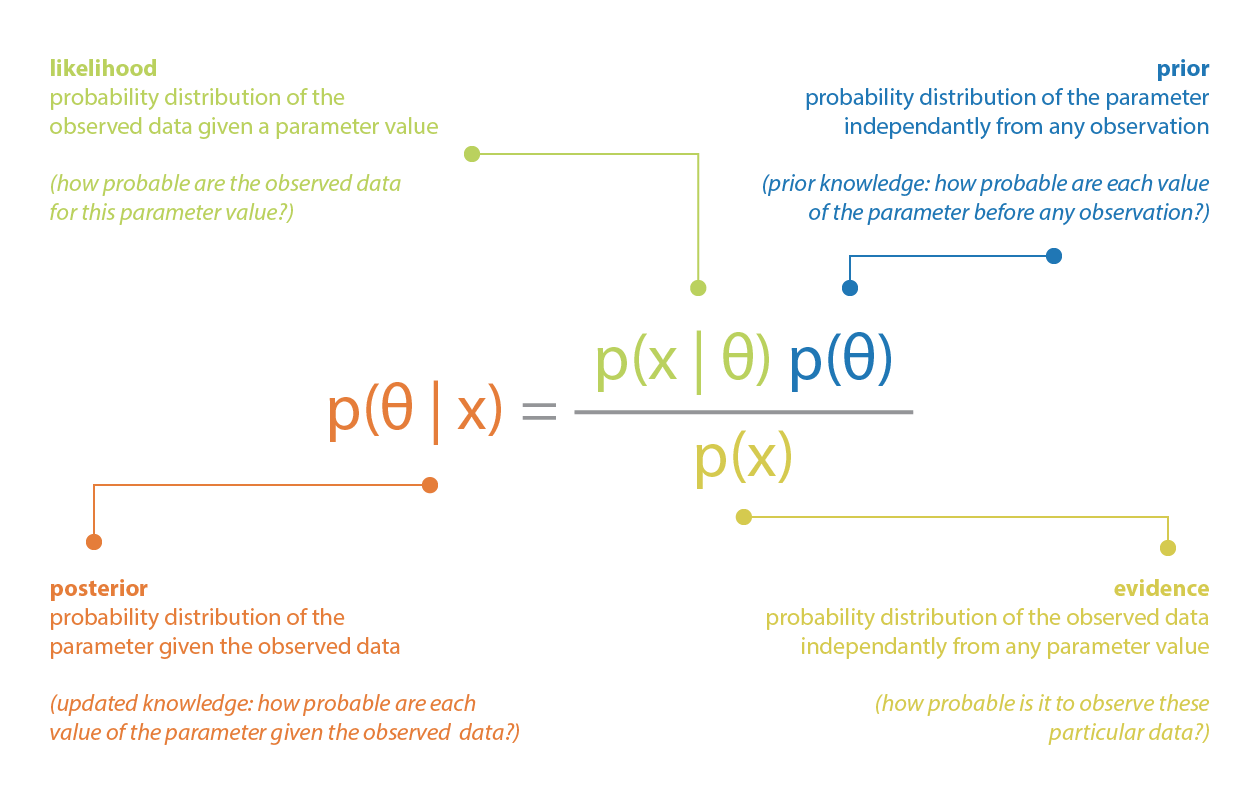
\includegraphics[width=.3\textwidth]{pic/p05c08-snip01}
    \caption{A supposed portrait of Thomas Bayes, an English statistician, philosopher, and theologian}
    \label{fig:p05c08-snip01}
\end{figure}

Computing some of these probabilities can be tedious, especially the evidence $P(D)$. Also, other problems can arise such as those of ensuring conjugacy which I will not dive into in this article. Luckily, some techniques, namely MCMC, allow us to sample from the posterior, and a draw distributions over our parameters without having to worry about computing the evidence, nor about conjugacy.

\subsection{Markov Chain Monte Carlo}
MCMC allows us to draw samples from a distribution even if we can't compute it. It can be used to sample from the posterior distribution (what we wish to know) over parameters. It has seen much success in many applications, such as computing the distribution of parameters given a set of observations and some prior belief, and also computing high dimensional integrals in physics and in digital communications.
Bottom line: It can be used to compute the distribution over the parameters given a set of observations and a prior belief.

\subsection{Metropolis-Hastings}
MCMC is a class of methods. Metropolis-Hastings is a specific implementation of MCMC. It works well in high dimensional spaces as opposed to Gibbs sampling and rejection sampling.

This technique requires a simple distribution called the proposal distribution (Which I like to call transition model) $Q(\theta^\prime/\theta)$ to help draw samples from an intractable posterior distribution $P(\theta =\theta/D)$.

Metropolis-Hastings uses $Q$ to randomly walk in the distribution space, accepting or rejecting jumps to new positions based on how likely the sample is. This "memoryless" random walk is the "Markov Chain" part of MCMC.

The "likelihood" of each new sample is decided by a function $f$. That's why $f$ must be proportional to the posterior we want to sample from. $f$ is commonly chosen to be a probability density function that expresses this proportionality.

To get a new position of the parameter, just take our current one, $\theta$, and propose a new one, $\theta^\prime$, that is a random sample drawn from $Q(\theta^\prime/\theta)$. Often this is a symmetric distribution. For instance, a normal distribution with mean $\theta$ and some standard deviation $\sigma$: $Q(\theta^\prime/\theta) = N(\theta, \sigma)$

To decide if $\theta^\prime$ is to be accepted or rejected, the following ratio must be computed for each new proposed $\theta^\prime$:
\begin{equation}\frac{P\left(\theta^{\prime} / D\right)}{P(\theta / D)}\end{equation}
Using Bayes' formula this can be easily re-formulated as:
\begin{equation}\frac{P\left(D / \theta^{\prime}\right) P\left(\theta^{\prime}\right)}{P(D / \theta) P(\theta)}\end{equation}
(the evidence $P(D)$ is simply crossed out during the division).
Which is also equivalent to:
\begin{equation}\frac{\prod_{i}^{n} f\left(d_{i} / \Theta=\theta^{\prime}\right) P\left(\theta^{\prime}\right)}{\prod_{i}^{n} f\left(d_{i} / \Theta=\theta\right) P(\theta)}\end{equation}
Where $f$ is the proportional function mentioned previously.

The rule for acceptance, can then be formulated as:
\begin{equation}
P(\text { accept })=\left\{
\begin{array}{ll}
\frac{\prod_{i}^{n} f\left(d_{i} / \Theta=\theta^{\prime}\right) P\left(\theta^{\prime}\right)}{\prod_{i}^{n} f\left(d_{i} / \Theta=\theta\right) P(\theta)}, & \Pi_{i}^{h} f\left(d_{i} / \Theta=\theta\right) P(\theta)>\Pi_{i}^{n} f\left(d_{i} / \Theta=\theta^{\prime}\right) P\left(\theta^{\prime}\right) \\
1,& \Pi_{i}^{n} f\left(d_{i} / \Theta=\theta\right) P(\theta) \leq \Pi_{i}^{n} f\left(d_{i} / \Theta=\theta^{\prime}\right) P\left(\theta^{\prime}\right)
\end{array}\right.
\end{equation}
Note: The prior components are often crossed if there is no preference or restrictions on the parameters.
This means that if a $\theta^\prime$ is more likely than the current $\theta$, then we always accept $\theta^\prime$. If it is less likely than the current $\theta$, then we might accept it or reject it randomly with decreasing probability, the less likely it is.

So, briefly, the Metropolis-Hastings algorithm does the following:

Given
\begin{itemize}[itemsep=-1ex]
\item $f$, the PDF of the distribution to sample from
\item $Q$, the transition model,
\item $\theta_{0}$, a first guess for $\theta$
\item $\theta=\theta_{0}$ 
\end{itemize}
for $n$ iterations:
\begin{itemize}[itemsep=-1ex]
\item $p=f(D / \Theta=\theta) P(\theta)$
\item $\theta^{\prime}=Q\left(\theta_{i}\right)$
\item $p^{\prime}=f\left(D / \Theta=\theta^{\prime}\right) P\left(\theta^{\prime}\right)$
\item ratio $=\frac{p^{\prime}}{p}$
\item generate a uniform random number $r$ in $[0,1]$
\item if $r<$ ratio:\\
\ \ \ $\operatorname{set} \theta_{i}=\theta^{\prime}$
\end{itemize}

\section{Part 2: Dummy data example}

\subsection{Step 1: Data generation}
We generate 30,000 samples from a normal distribution with mean  $\mu$=10, and standard deviation $\sigma$=3, but we can only observe 1000 random samples from them.
\begin{lstlisting}
mod1=lambda t:np.random.normal(10,3,t)

#Form a population of 30,000 individual, 
#with average=10 and scale=3
population = mod1(30000)
#Assume we are only able to observe 1,000 of these individuals.
observation = population[np.random.randint(0, 30000, 1000)]

fig = plt.figure(figsize=(10,10))
ax = fig.add_subplot(1,1,1)
ax.hist( observation,bins=35 ,)
ax.set_xlabel("Value")
ax.set_ylabel("Frequency")
ax.set_title("Figure 1: Distribution of 1000 observations"
" sampled from a population of 30,000 with mu=10, sigma=3")
mu_obs=observation.mean()
mu_obs
\end{lstlisting}


\begin{figure}[h]
    \centering
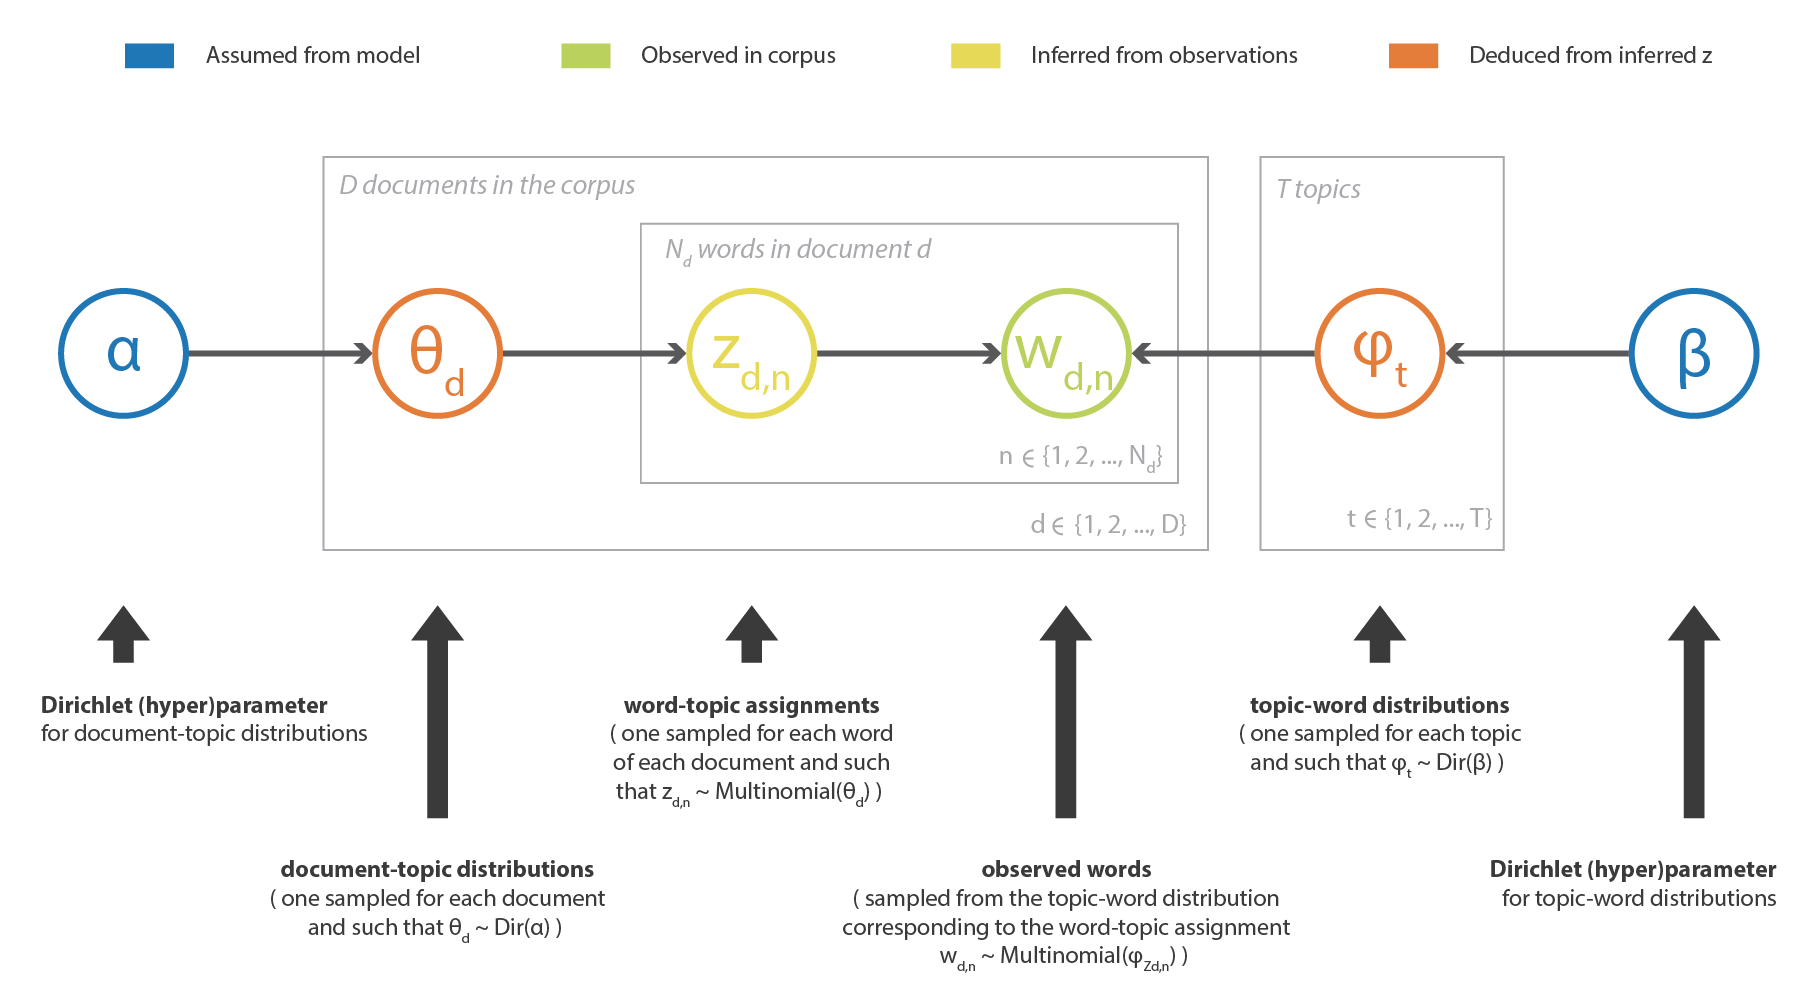
\includegraphics[width=.6\textwidth]{pic/p05c08-snip02}
    \caption{Samples from normal distribution}
    \label{fig:p05c08-snip02}
\end{figure}


\subsection{Step 2: What do we want?}
We would like to find a distribution for $\sigma_\textrm{observed}$ using the 1000 observed samples. Those of you who are avid mathematicians will say that there is a formula for computing $\sigma$:
\begin{equation}
\sigma=\sqrt{\frac{1}{n} \sum_{i}^{n}\left(d_{i}-\mu\right)^{2}}
\end{equation}
Why do we want to sample and whatnot? Well, this is just a dummy data example, the real problem is in part 3, where it's hard to compute the parameters directly. Plus here, we are not trying to find a value for $\sigma$, but rather, we are trying to compute a probability distribution for $\sigma$.

\subsection{Step 3: Define the PDF and the transition model}
From Figure~\ref{fig:p05c08-snip02}, we can see that the data is normally distributed. The mean can be easily computed by taking the average of the values of the 1000 samples. By doing that, we get that  $\mu_\textrm{observed}$ = 9.8 (although on a side note, we could have also assumed  $\mu$ to be unknown and sampled for it just like we are doing for $\sigma$. However, I want to make this starting example simple.)

\textbf{For the transition model/ proposal distribution}

I have no specific distribution in mind, so I will choose a simple one: the Normal distribution!
\begin{equation}Q\left(\sigma_{\text {new}} / \sigma_{\text {current}}\right)=N\left(\mu=\sigma_{\text {current},} \sigma^{\prime}=1\right)\end{equation}
Note that  $\sigma^\prime$ is unrelated to $\sigma_\textrm{new}$ and $\sigma_\textrm{current}$. It simply specifies the standard deviation of the parameter space. It can be any value desired. It affects the convergence time of the algorithm and the correlation between samples, which I talk about later.

\textbf{For the PDF}

Since $f$ should be proportional to the posterior, we choose $f$ to be the following Probability Density Function (PDF), for each data point di in the data set D:
\begin{equation}f\left(d_{i} / \mu, \sigma^{2}\right)=\frac{1}{\sqrt{2 \pi \sigma^{2}}} e^{-\frac{\left(d_{i}-\mu\right)^{2}}{2 \sigma^{2}}}\end{equation}
In our case, $\theta$ is made up of two values: $[\mu, \sigma],$ and that $\mu$ is a constant, $\mu=\mu_\textrm{observed}$.
Since  $\mu$ is constant, we can practically consider that $\sigma$ is equivalent to $\theta$.

\subsection{Step 4: Define when we accept or reject $\sigma_\textrm{new}$}

\textbf{The acceptance formula}
We accept $\sigma_\textrm{new}$ if 
\begin{equation}\frac{\text {Likelihood}\left(\boldsymbol{D} / \mu_{\text {obs}}, \sigma_{\text {new}}\right) * \text {prior}\left(\boldsymbol{\mu}_{\text {obs}}, \boldsymbol{\sigma}_{\text {new}}\right)}{\text {Likelihood}\left(\boldsymbol{D} / \mu_{\text {obs}}, \boldsymbol{\sigma}_{\text {current}}\right) * \text { prior}\left(\boldsymbol{\mu}_{\text {obs}}, \sigma_{\text {current}}\right)}>1
\label{eq:equation01}
\end{equation}

If this ratio is not larger than 1, then we compare it to a uniformly generated random number in the closed set [0,1]. If the ratio is larger than the random number, we accept $\sigma_\textrm{new}$, otherwise we reject it. This ensures that even if a sample is less likely than the current, we might still want to try it. (Similar notion to simulated annealing).

\textbf{The likelihood}

The total likelihood for a set of observation $D$ is:
\begin{equation}\text {Likelihood}\left(\boldsymbol{D} / \mu_{\text {obs}}, \boldsymbol{\sigma}_{a}\right)=\prod_{i}^{n} f\left(d_{i} / \mu_{\text {obs}}, \sigma_{a}\right), \text { where } a=\text {new or current.}\end{equation}
This must be computed for both new and current sigma in order to compute the ratio in Equation~\ref{eq:equation01}.

\textbf{The Prior $P(\mu,\sigma)$}

We don't have any preferences for the values that $\sigma_\textrm{new}$ and $\sigma_\textrm{current}$ can take. The only thing worth noting is that they should be positive. Why? Intuitively, the standard deviation measures dispersion. Dispersion is a distance, and distances cannot be negative.
Mathematically:
\begin{equation}\sigma=\sqrt{\frac{1}{n} \sum_{i}^{n}\left(d_{i}-\mu\right)^{2}}\end{equation}
and the square root of a number cannot be negative, so $\sigma$ is always positive. We strictly enforce this in the prior.

\textbf{The final acceptance form}

In our case, we will log both the prior and the likelihood function. Why log? Simply because it helps with numerical stability, i.e. multiplying thousands of small values (probabilities, likelihoods, etc.) can cause an underflow in the system's memory, and the log is a perfect solution because it transforms multiplications to additions and transforms small positive numbers into non-small negative numbers.
Our acceptance condition from Equation~\ref{eq:equation01} becomes:
\begin{itemize}
\item Accept $\sigma_{\text {new}}$ if:\\
$\log\left(\text {Likelihood}\left(D / \mu_{\text {obs},}, \sigma_{\text {new}}\right)\right)+\log \left(\text {prior}\left(\mu_{\text {obs}}, \sigma_{\text {new}}\right)\right)$\\
$-\left(\log\left(\text {Likelihood}\left(D / \mu_{\text {obs}}, \sigma_{\text {current}}\right)\right)+\right.$
$\left.\log \left(\text {prior}\left(\mu_{\text {obs}}, \sigma_{\text {current}}\right)\right)\right)$\\
$>0$

\item Equivalent to:\\
$\sum_{i}^{n} \log \left(f\left(d_{i} / \mu_{\text {obs}}, \sigma_{\text {new}}\right)\right)+\log \left(\text {prior}\left(\mu_{\text {obs}}, \sigma_{\text {new}}\right)\right)-\Sigma_{i}^{n} \log \left(f\left(d_{i} / \mu_{\text {obs}}, \sigma_{\text {current}}\right)\right)$\\
$-\log \left(\text {prior}\left(\mu_{\text {obs}}, \sigma_{\text {current}}\right)\right)$\\
$>0$

\item Equivalent to:\\
$\Sigma_{i}^{n} \log \left(f\left(d_{i} / \mu_{\text {obs}}, \sigma_{\text {new}}\right)\right)+\log \left(\text {prior}\left(\mu_{\text {obs}}, \sigma_{\text {new}}\right)\right)$\\
$>\Sigma_{i}^{n} \log \left(f\left(d_{i} / \mu_{\text {obs}}, \sigma_{\text {current}}\right)\right)+\log \left(\text {prior}\left(\mu_{\text {obs}}, \sigma_{\text {current}}\right)\right)$

\item Equivalent to:\\
$\Sigma_{i}^{n}
-n \log \left(\sigma_{new} \sqrt{2 \pi}\right)
-\frac{\left(d_{i}-\mu_{obs}\right)^{2}}{2 \sigma_{new}^{2}}+
\log\left(prior\left(\mu_{obs}, \sigma_{new}\right)\right)>$
$$
\Sigma_{i}^{n}-n \log \left(\sigma_{\text {current }} \sqrt{2 \pi}\right)-\frac{\left(d_{i}-\mu_{\text {obs }}\right)^{2}}{2 \sigma_{\text {current }}}^{2}+\log\left(\text { prior }\left(\mu_{\text {obs }}, \sigma_{\text {current }}\right)\right)
$$
\end{itemize}


This form can be reduced even more by taking the square root and the multiplication out of the log, but never mind that now, there's already enough maths!

\textbf{The implementation of that rant}

\begin{lstlisting}
#The transition model defines how to move from sigma_current to sigma_new
transition_model = lambda x: [x[0],np.random.normal(x[1],0.5,(1,))]

def prior(x):
    #x[0] = mu, x[1]=sigma (new or current)
    #returns 1 for all valid values of sigma. Log(1) =0, so it does not affect the summation.
    #returns 0 for all invalid values of sigma (<=0). Log(0)=-infinity, and Log(negative number) is undefined.
    #It makes the new sigma infinitely unlikely.
    if(x[1] <=0):
        return 0
    return 1

#Computes the likelihood of the data given a sigma (new or current) according to equation (2)
def manual_log_like_normal(x,data):
    #x[0]=mu, x[1]=sigma (new or current)
    #data = the observation
    return np.sum(-np.log(x[1] * np.sqrt(2* np.pi) )-((data-x[0])**2) / (2*x[1]**2))

#Same as manual_log_like_normal(x,data), but using scipy implementation. It's pretty slow.
def log_lik_normal(x,data):
    #x[0]=mu, x[1]=sigma (new or current)
    #data = the observation
    return np.sum(np.log(scipy.stats.norm(x[0],x[1]).pdf(data)))


#Defines whether to accept or reject the new sample
def acceptance(x, x_new):
    if x_new>x:
        return True
    else:
        accept=np.random.uniform(0,1)
        # Since we did a log likelihood, we need to exponentiate in order to compare to the random number
        # less likely x_new are less likely to be accepted
        return (accept < (np.exp(x_new-x)))


def metropolis_hastings(likelihood_computer,prior, transition_model, param_init,iterations,data,acceptance_rule):
    # likelihood_computer(x,data): returns the likelihood that these parameters generated the data
    # transition_model(x): a function that draws a sample from a symmetric distribution and returns it
    # param_init: a starting sample
    # iterations: number of accepted to generated
    # data: the data that we wish to model
    # acceptance_rule(x,x_new): decides whether to accept or reject the new sample
    x = param_init
    accepted = []
    rejected = []   
    for i in range(iterations):
        x_new =  transition_model(x)    
        x_lik = likelihood_computer(x,data)
        x_new_lik = likelihood_computer(x_new,data) 
        if (acceptance_rule(x_lik + np.log(prior(x)),x_new_lik+np.log(prior(x_new)))):            
            x = x_new
            accepted.append(x_new)
        else:
            rejected.append(x_new)            
                
    return np.array(accepted), np.array(rejected)
\end{lstlisting}
The implementation is quite simple, right ?!

\subsection{Step 6: Run the algorithm with initial parameters and collect accepted and rejected samples}

\begin{lstlisting}
accepted, rejected = metropolis_hastings(manual_log_like_normal,prior,transition_model,[mu_obs,0.1], 50000,observation,acceptance)
\end{lstlisting}

The algorithm accepted 8317 samples (which might be different on each new run). The last 10 samples contain the following values for $\sigma$:\newline
[2.87920187, 3.10388928, 2.94469786, 3.04094103, 2.95522153, 3.09328088, 3.07361275, 3.08588388, 3.12881964, 3.03651136]\newline
Let's see how the algorithm worked its way to these values:

\begin{figure}[h]
    \centering
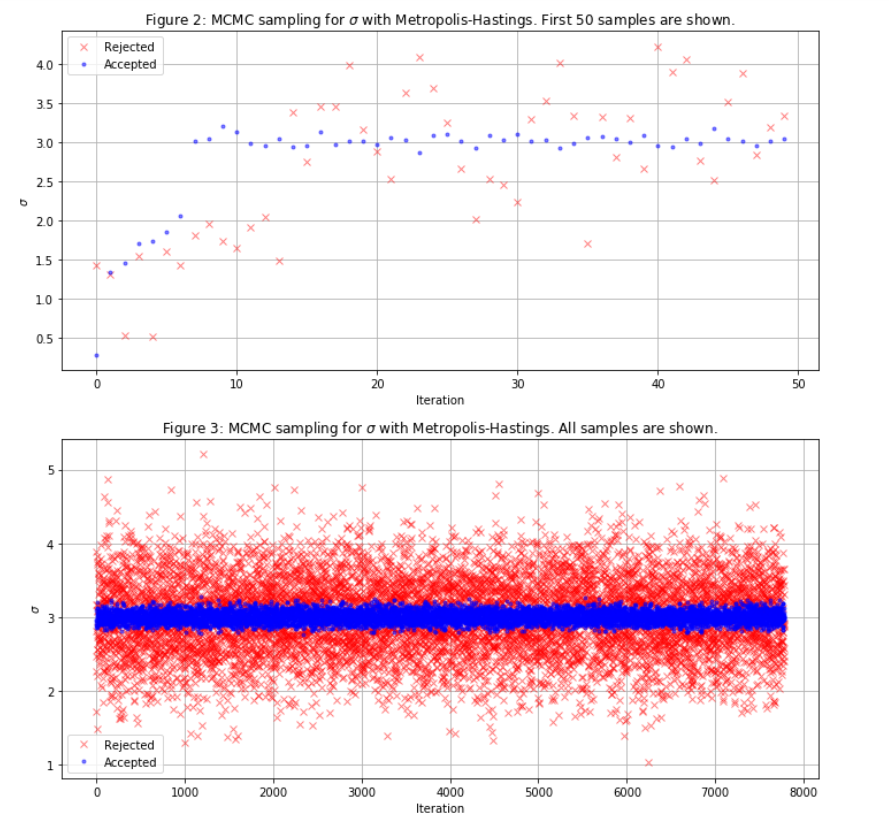
\includegraphics[width=.6\textwidth]{pic/p05c08-snip03}
    \caption{Run results}
    \label{fig:p05c08-snip03}
\end{figure}

So, starting from an initial $\sigma$ of 0.1, the algorithm converged pretty quickly to the expected value of 3. That said, it's only sampling in a 1D space. so it's not very surprising.
Still, we will consider the initial 25\% of the values of $\sigma$ to be "burn-in", so we drop them.

\textbf{Let's visualise the trace of $\sigma$ and the histogram of the trace}


\begin{figure}[h]
    \centering
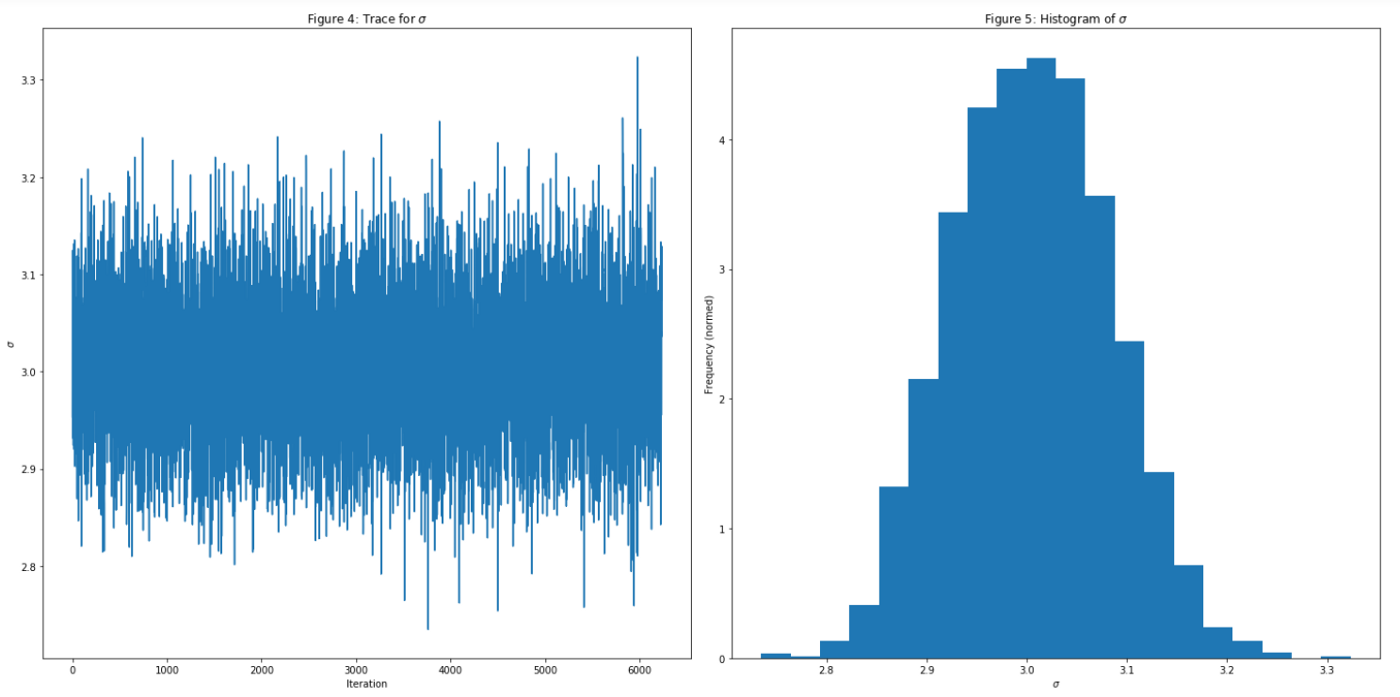
\includegraphics[width=.6\textwidth]{pic/p05c08-snip04}
    \caption{The trace and histogram}
    \label{fig:p05c08-snip04}
\end{figure}


The most likely value for $\sigma$ is around 3.1. This is a wee bit more than the original value of 3.0. The difference is due to us observing only 3.33\% of the original population (1,000 out of 30,000)

\textbf{Predictions: How would our model fare in predicting the original population of 30,000?}

First, we average the last 75\% of accepted samples of $\sigma$, and we generate 30,000 random individuals from a normal distribution with  $\mu$=9.8 and $\sigma$=3.05 (the average of the last 75\% of accepted samples) which is actually better than the most likely value of 3.1.

\begin{figure}[h]
    \centering
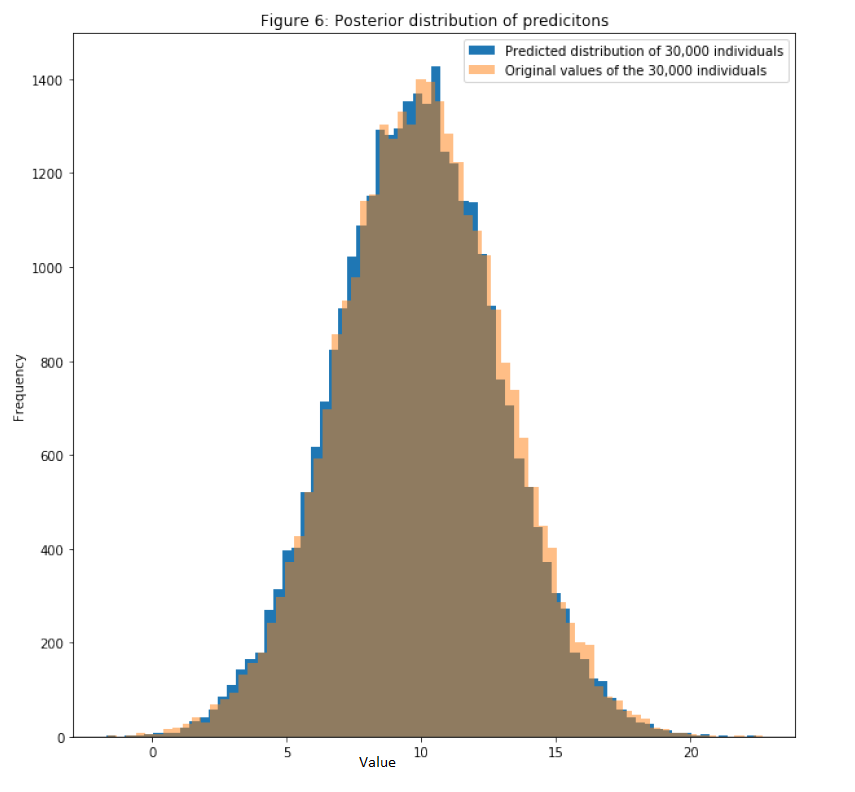
\includegraphics[width=.6\textwidth]{pic/p05c08-snip05}
    \caption{The histogram for 30,000 samples}
    \label{fig:p05c08-snip05}
\end{figure}

\section{Part 3: A real world example}

\begin{figure}[h]
    \centering
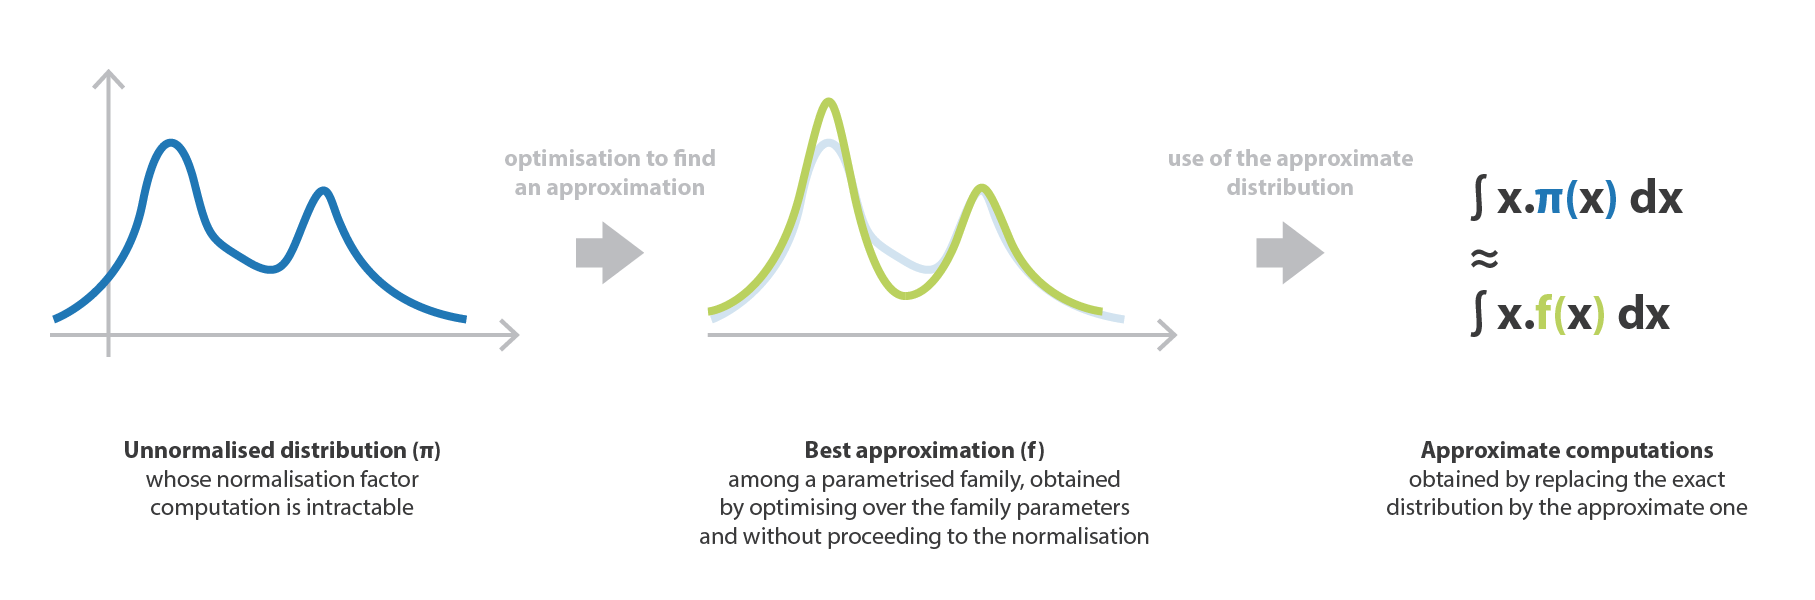
\includegraphics[width=.6\textwidth]{pic/p05c08-snip06}
    \caption{Sun spots}
    \label{fig:p05c08-snip06}
\end{figure}

A sunspot is a region on the Sun's surface (photo-sphere) that is marked by a lower temperature than its environment. These reduced temperatures are caused by concentrations of magnetic field flux that inhibit convection by an effect similar to eddy current brakes. Sunspots usually appear in pairs of opposite magnetic polarity. Their number varies according to the approximately 11-year solar cycle.

The data we will be working on is the "Monthly mean total sunspot number", for each month from January 1749 to November 2018. This data is collected, curated and made publicly available by the World Data Center for the production, preservation and dissemination of the international sunspot number.

\subsection{Let's plot the data over the years to see what the distribution might be like}

\begin{figure*}[h]
    \centering
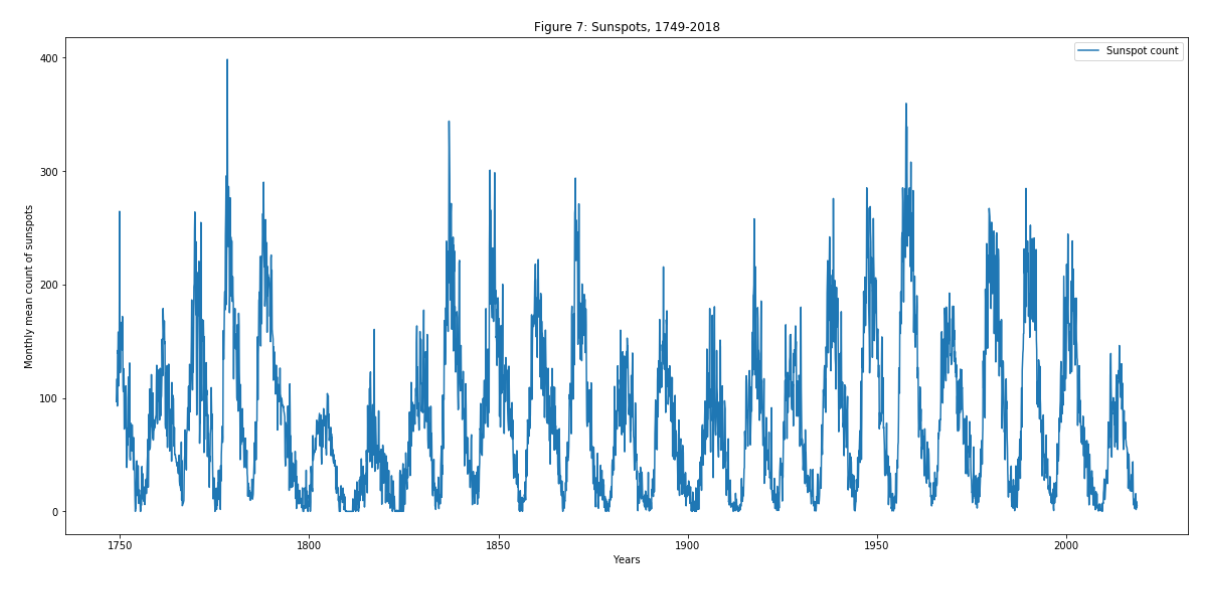
\includegraphics[width=.48\textwidth]{pic/p05c08-snip07}
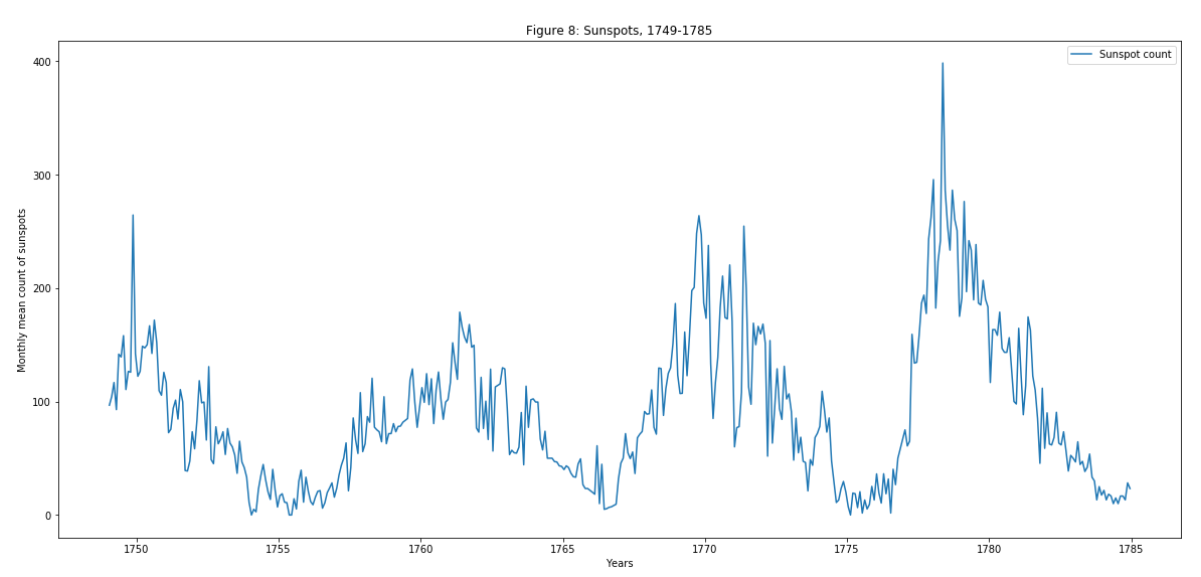
\includegraphics[width=.48\textwidth]{pic/p05c08-snip08}
    \caption{Sun spot cycles}
    \label{fig:p05c08-snip07}
\end{figure*}

\FloatBarrier

\subsection{Modelling sun spots}
It seems like we could model this phenomenon with a gamma distribution, with a new cycle resetting every 12 years
A gamma distribution  $\Gamma$ is a two-parameter family of continuous probability distributions. The parameters are the shape a and the scale b. A random variable X that is gamma-distributed is noted X~ $\Gamma$(a, b), and in our case X is the count of sunspots. The two parameters a and b are the unknowns that we would like to calculate distributions for.

\begin{figure}[h]
    \centering
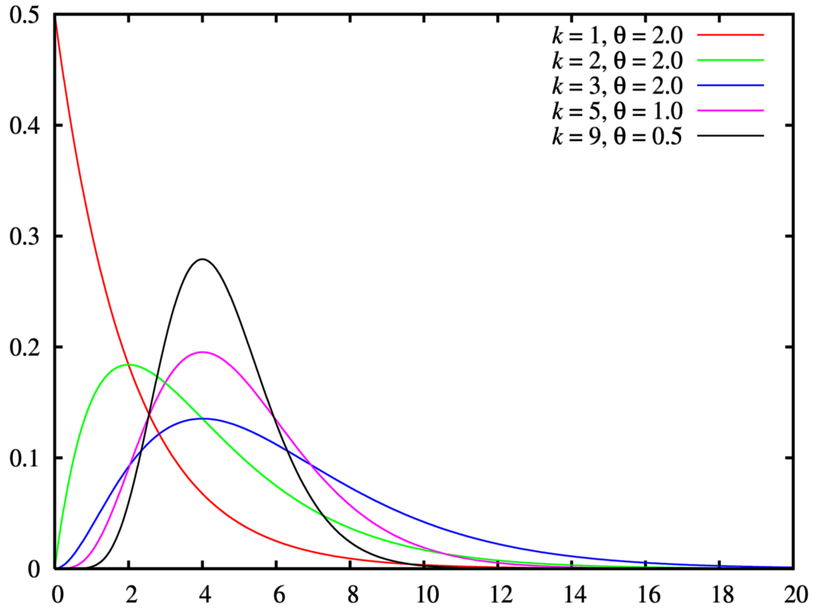
\includegraphics[width=.6\textwidth]{pic/p05c08-snip09}
    \caption{Gamma function with different parameters}
    \label{fig:p05c08-snip09}
\end{figure}

For example, in the first cycle, the sunspot counts start from their highest at about 300 at the end of 1749, and fall to their lowest 6 years after, during 1755. Then the number rises up again to it's maximum during 1761 and 1762 before falling again during 1766 and so on.

\begin{figure}[h]
    \centering
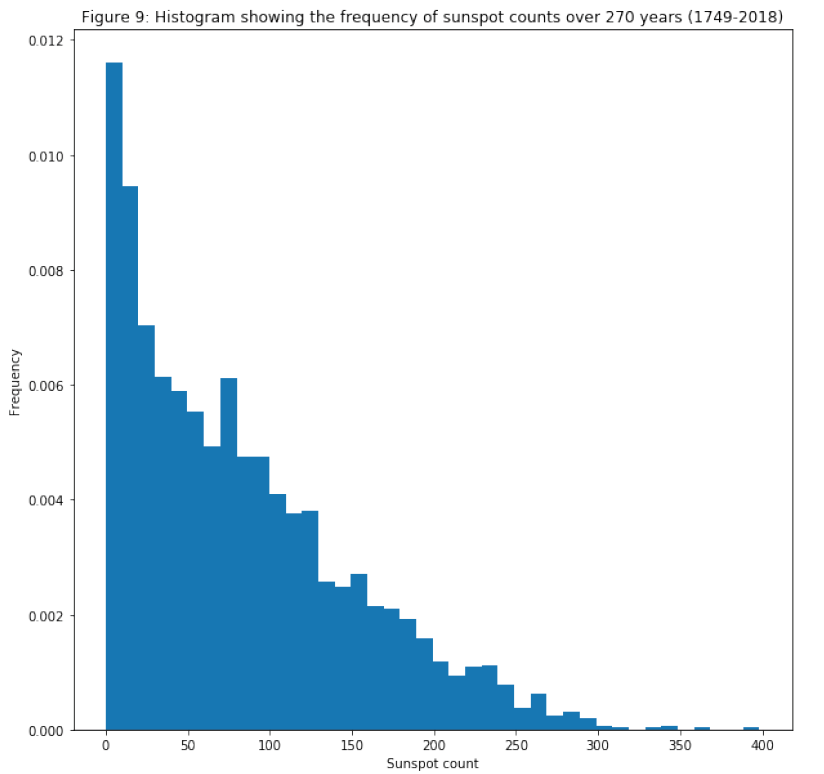
\includegraphics[width=.6\textwidth]{pic/p05c08-snip10}
    \caption{Histogram of sunspot counts}
    \label{fig:p05c08-snip10}
\end{figure}

\FloatBarrier
\subsection{Gamma distribution}
Indeed, it does seem like the frequency of counts follows a gamma distribution
The gamma distribution, has for PDF, f such that:
\begin{equation}f(x ; a, b)=\frac{b^{a} x^{a-1} e^{-b x}}{\Gamma(a)}\end{equation}
where  $\Gamma$ is the gamma function:  $\Gamma$(a) = (a-1)! (not to be confused with the gamma distribution).

Following the same procedure as in the dummy data example, we can write down the log likelihood from this pdf (see code below). Alternatively, one could use the \lstinline{scipy.stats.gamma(a, b).pdf(x)} function to compute it. However, beware that scipy's implementation is several orders of magnitudes slower than the one I implemented.

Since $a$ and $b$ must be strictly positive, we enforce this in the prior:

\begin{lstlisting}
transition_model = lambda x: np.random.normal(x,[0.05,5],(2,))
import math
def prior(w):
    if(w[0]<=0 or w[1] <=0):
        return 0
    else:
        return 1
    
def manual_log_lik_gamma(x,data):
    return np.sum((x[0]-1)*np.log(data) - (1/x[1])*data - x[0]*np.log(x[1]) - np.log(math.gamma(x[0])))
    
def log_lik_gamma(x,data):
    return np.sum(np.log(scipy.stats.gamma(a=x[0],scale=x[1],loc=0).pdf(data)))    
\end{lstlisting}

Run the code and collect samples:
\begin{lstlisting}
accepted, rejected = metropolis_hastings(manual_log_lik_gamma,prior,transition_model,[4, 10], 50000,activity,acceptance)
\end{lstlisting}
Starting from $a$=4, and $b$=10, the algorithm accepted 8561 pairs of samples, the last value for $a$ is 0.98848982 and the last value for $b$ is 84.99360422, which are pretty far off the initial values.

As with the dummy data example, let's see how the algorithm worked its way to these values:

\begin{figure}[h]
    \centering
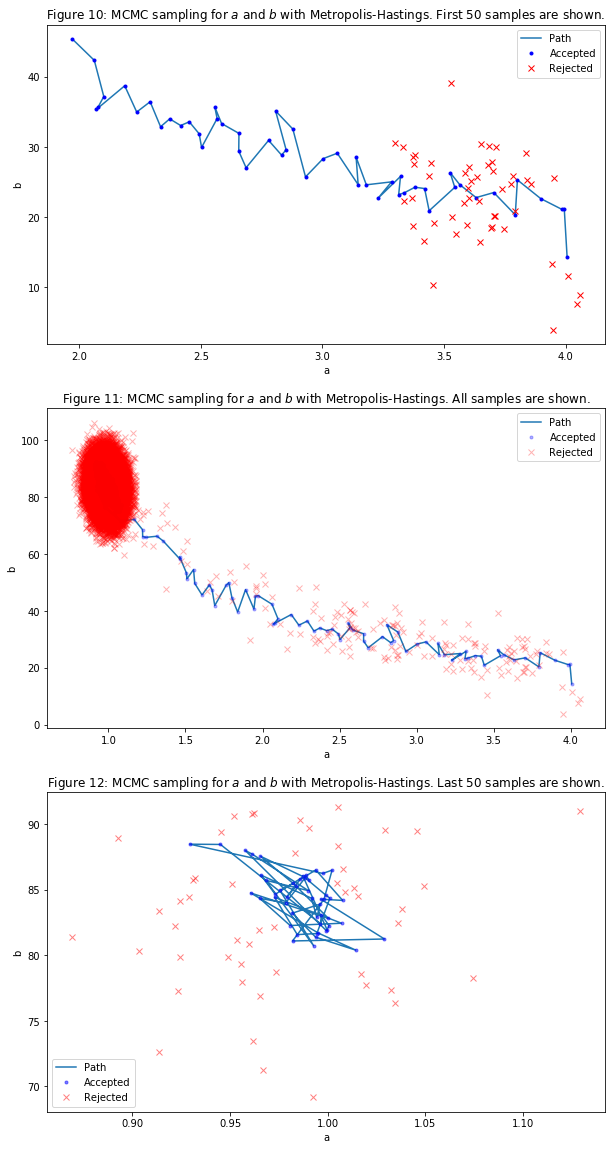
\includegraphics[width=.8\textwidth]{pic/p05c08-snip11}
    \caption{MCMC solution for $a$ and $b$}
    \label{fig:p05c08-snip11}
\end{figure}

As we can see from the figures, the algorithm converges quickly to the [$a$=1,$b$=85] zone.

Tip: when the algorithm starts to heavily reject samples, that means that we have reached a zone of saturation of the likelihood. Commonly, this can be interpreted as having reached the optimal parameter space from which we can sample, i.e. there is very little reason for the algorithm to accept new values. This is marked in figures 11, and 12 where the algorithm no longer accepts any values outside of a small range.

\textbf{Burn-in}

We consider the initial 50\% of the values of a and b to be "burn-in", so we drop them. Let's visualise the traces of and b and the histogram of the traces.


\begin{figure}[h]
    \centering
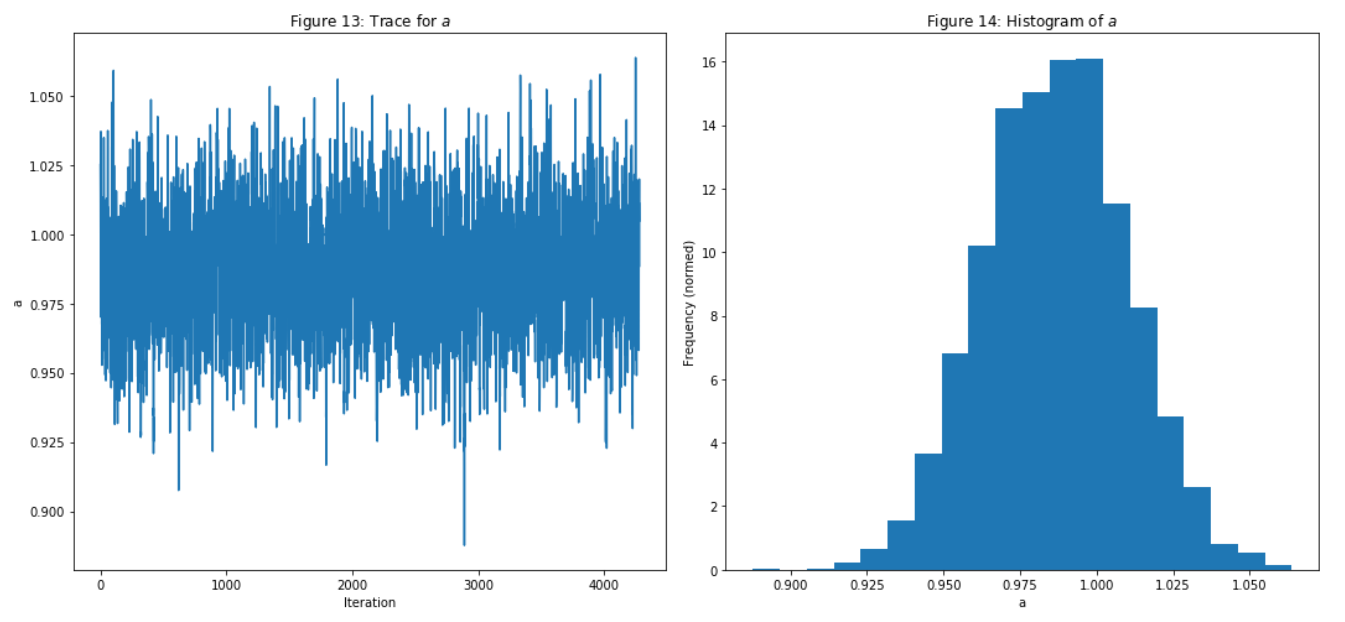
\includegraphics[width=.8\textwidth]{pic/p05c08-snip12}
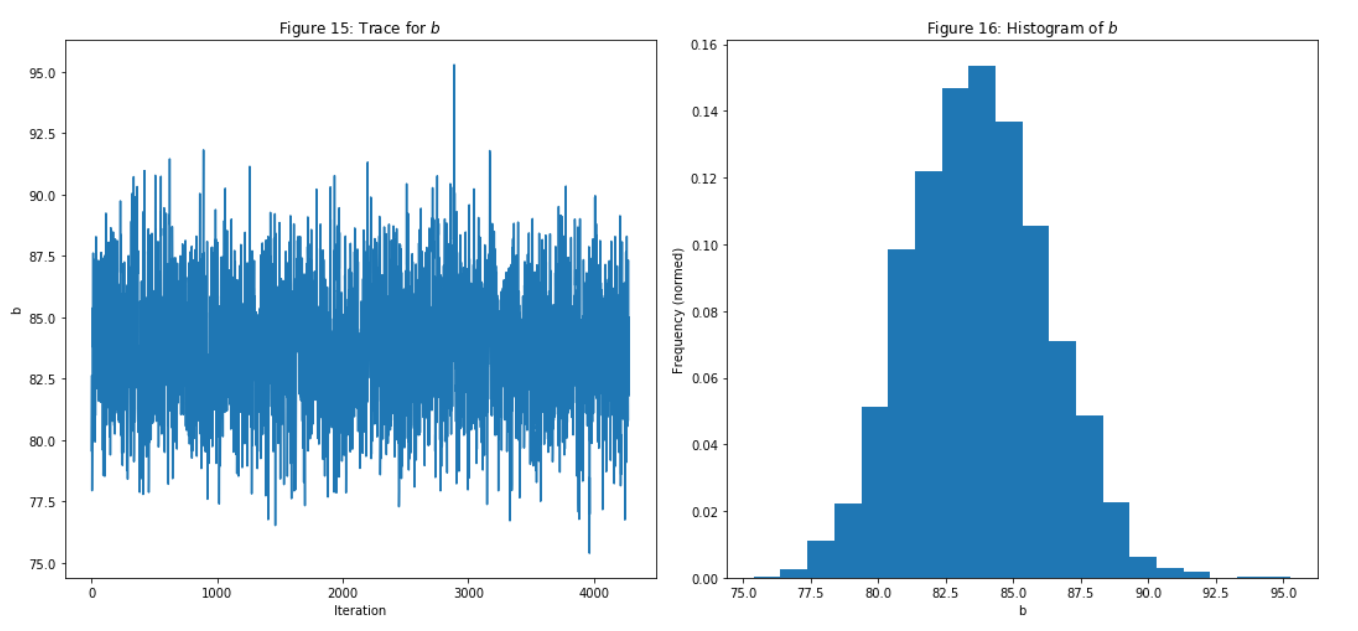
\includegraphics[width=.8\textwidth]{pic/p05c08-snip13}
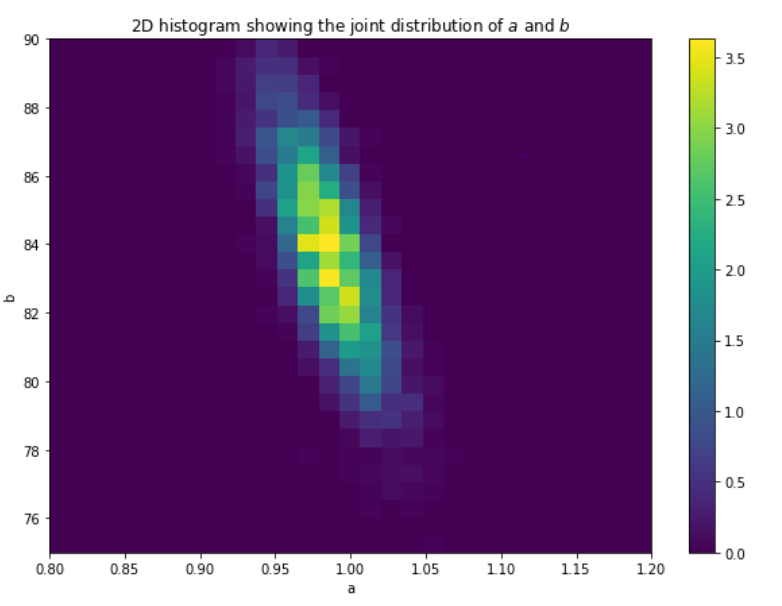
\includegraphics[width=.8\textwidth]{pic/p05c08-snip14}
    \caption{Trace histogram}
    \label{fig:p05c08-snip12}
\end{figure}


\subsection{Prediction time}
First, we average the last 50\% of accepted samples of a and b, and we generate random individuals from a  $\Gamma$ distribution. $a_\textrm{average}$=0.9866200759935773 and $b_\textrm{average}$=83.70749712447888.
And the predictions:

\begin{figure}[h]
    \centering
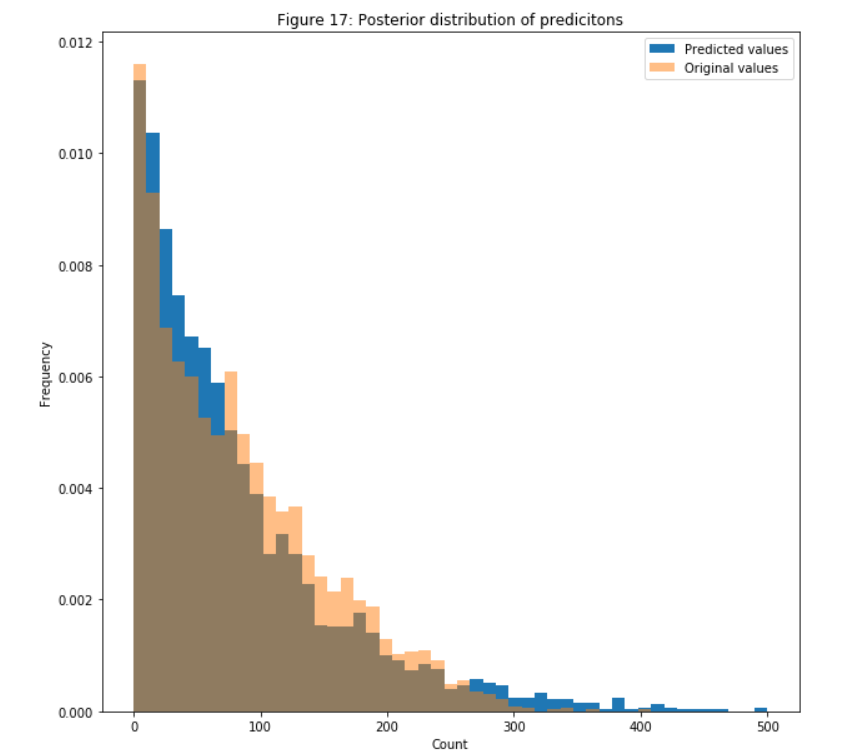
\includegraphics[width=.8\textwidth]{pic/p05c08-snip15}
    \caption{Predictions}
    \label{fig:p05c08-snip15}
\end{figure}

\FloatBarrier
\section{Evaluation}
\subsection{Evaluation of the proposal distribution}
How do we specify the parameters for the distribution Q? Should we move far from the current sample $\theta$, or stay relatively close? These questions can be answered by measuring the auto-correlation between accepted samples. We don't want distant samples to be too correlated as we are trying to implement a Markov Chain, i.e. a sample should only depend on its previous sample, and the auto-correlation plot should show a quick, exponential decrease between the correlation of sample $i$ and $i$-1,$i$-2,$\ldots$,$i$-$k$.

The auto-correlation is defined by computing the following function for each lag $k$:
\begin{equation}r_{k}=\frac{\sum_{i=1}^{N-k}\left(Y_{i}-Y_{a v g}\right)\left(Y_{i+k}-Y_{a v g}\right)}{\sum_{i=1}^{N}\left(Y_{i}-Y_{a v g}\right)^{2}}\end{equation}
The lag $k$, is  the range ahead of sample  $Y_i$ in which we would like to measure the correlation.

The plots below show the auto-correlation for $a$, $b$ for $k$ going from 1 to 100. A lag of $k$=0 means that we are measuring the correlation of a sample with itself, so we expect it to be equal to 1. The higher $k$ goes, the lower that correlation ought to be.
\begin{figure}[h]
    \centering
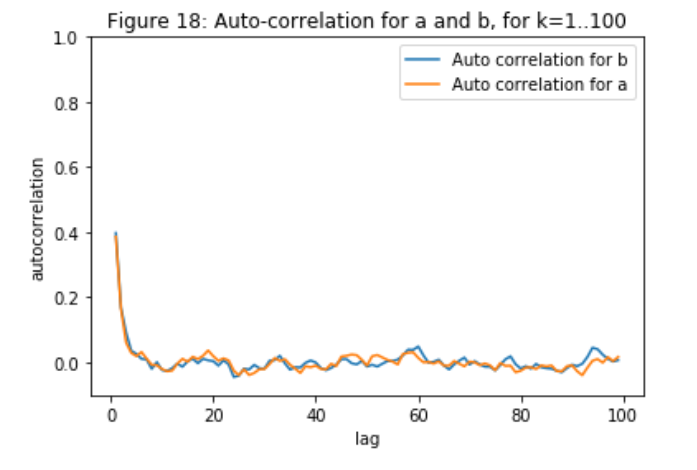
\includegraphics[width=.8\textwidth]{pic/p05c08-snip16}
    \caption{Auto-correlation of $a$ and $b$}
    \label{fig:p05c08-snip16}
\end{figure}
In our case, we are lucky to have a low enough correlation. In general, we might want to setup the parameters of the proposal distribution, $Q$, automatically. A common method is to keep adjusting the proposal parameters so that more than 50\% proposals are rejected. Alternatively, one could use an enhanced version of MCMC called Hamiltonian Monte Carlo, which reduces the correlation between successive sampled states and reaches the stationary distribution quicker.

\section{Conclusion}
While the abstraction behind this algorithm may seem out of grasp at first, the implementation is actually pretty simple, and gives awesome results. In fact, the great thing about probabilistic programming, notably MCMC is that you only need to write down the model and then run it. There is no need to compute the evidence, or ensure some constraining mathematical properties.

References \cite{PeterDriscoll2006,CarsonChow2010,GirolamiRogers2017}

